%!TEX root = ../paper.tex

% Small differences in anisotropy  
	In \cref{s:results} some differences in anisotropy of the kernels were observed, however these differences were relatively small. This section investigates the anisotropy of the kernels. 
	
		% Single Sphere
			\begin{figure}
				\centering
				\begin{subfigure}{0.23\textwidth}
					\centering
					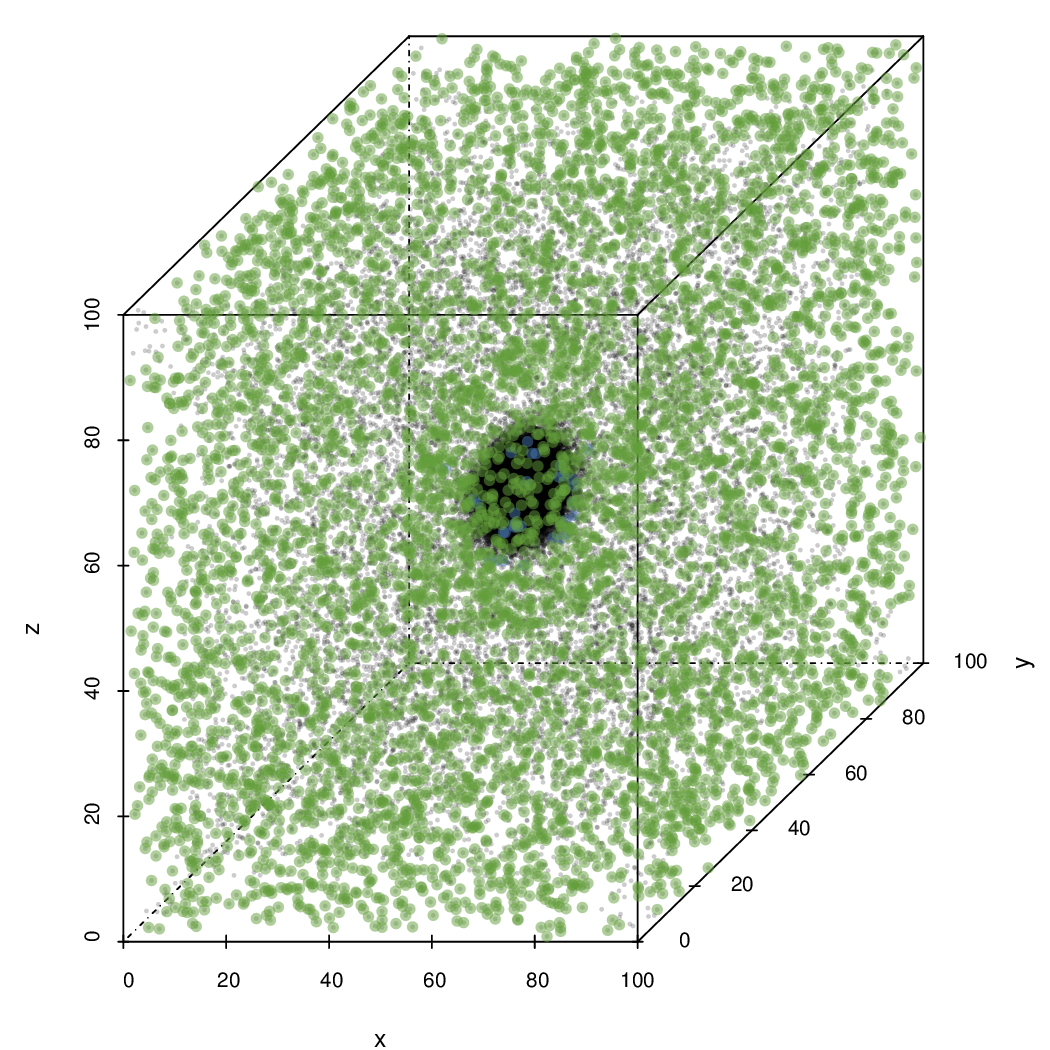
\includegraphics[keepaspectratio=true, width=\textwidth, height=0.23\textheight]{discussion/img/ferdosi_1_60000_anisotropy.png}
					\caption{\ferdosiOne [\num{2.783732800937043e+00}, \num{4.876641609906343e+00}]}
					\label{fig:discussion:anisotropy:ferdosi1}
				\end{subfigure}
				\begin{subfigure}{0.23\textwidth}
					\centering
					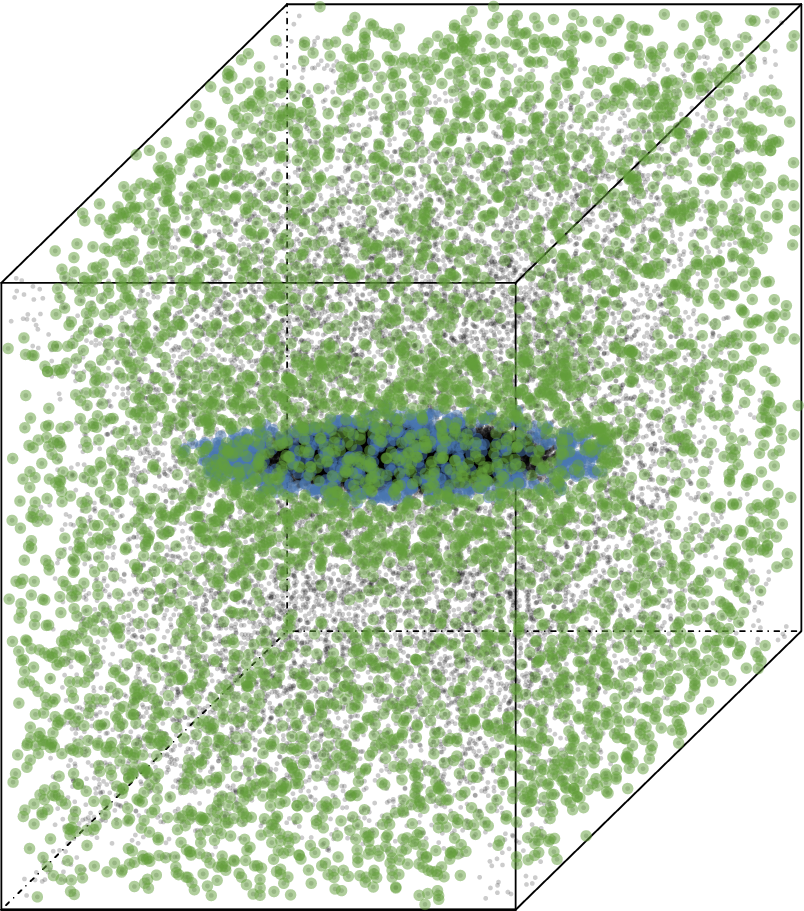
\includegraphics[keepaspectratio=true, width=\textwidth, height=0.23\textheight]{discussion/img/baakman_1_60000_anisotropy.png}
					\caption{\baakmanOne [\num{2.955638611296131e+00}, \num{4.876641609906340e+00}]}
					\label{fig:discussion:anisotropy:baakman1}
				\end{subfigure}	
				\begin{subfigure}{0.23\textwidth}
					\centering
					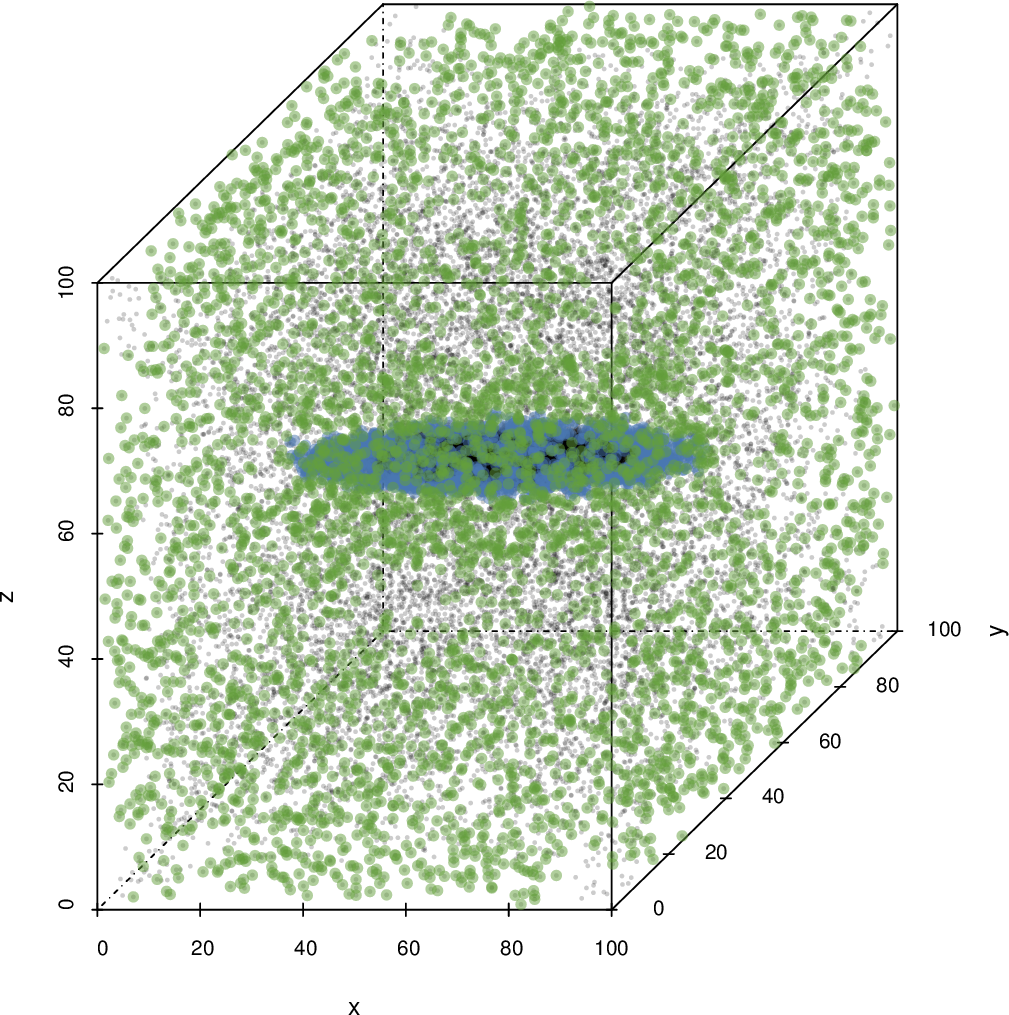
\includegraphics[keepaspectratio=true, width=\textwidth, height=0.23\textheight]{discussion/img/baakman_4_60000_anisotropy.png}
					\caption{\baakmanFour [\num{3.105833113039985e+00}, \num{5.987200775539245e+00}]}
					\label{fig:discussion:anisotropy:baakman4}
				\end{subfigure}		
				\begin{subfigure}{0.23\textwidth}
					\centering
					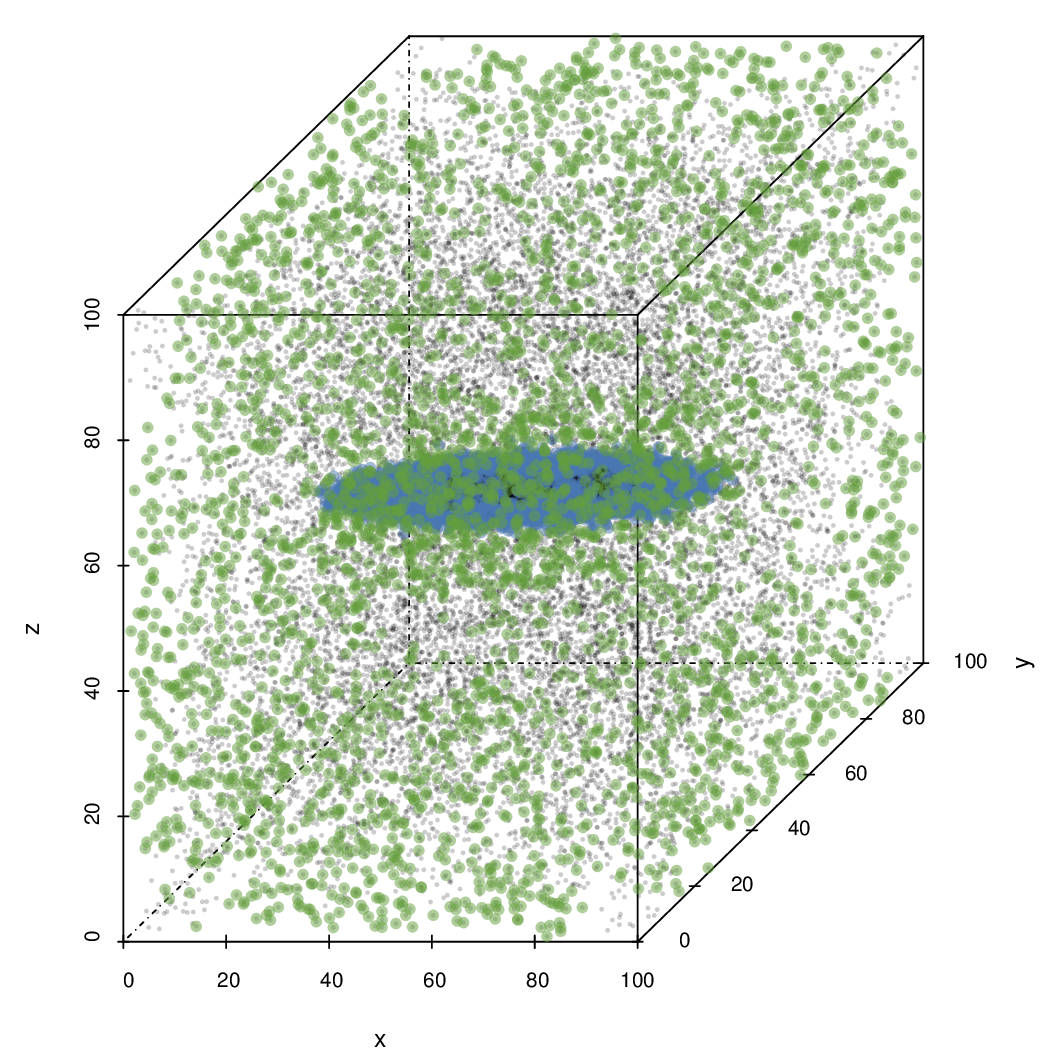
\includegraphics[keepaspectratio=true, width=\textwidth, height=0.23\textheight]{discussion/img/baakman_5_60000_anisotropy.png}
					\caption{\baakmanFive [\num{3.546238846198991e+00}, \num{8.192210308245695e+00}]}
					\label{fig:discussion:anisotropy:baakman5}
				\end{subfigure}			
				\caption{Scatter plot of the data sets
					\subref{fig:discussion:anisotropy:ferdosi1} \ferdosiOne, %
					\subref{fig:discussion:anisotropy:baakman1} \baakmanOne, %
					\subref{fig:discussion:anisotropy:baakman4} \baakmanFour, and %
					\subref{fig:discussion:anisotropy:baakman5} \baakmanFive. %
					The points with kernels whose anisotropy lies in the \nth{90} percentile are shown larger and in the color of the component they were drawn from. The range of the anisotropy of the kernels of the emphasized points in shown below each plot.}
				\label{fig:discussion:anisotropy:singleSphere}
			\end{figure}
			%	
			\Cref{fig:discussion:anisotropy:singleSphere} shows the datasets with a single Gaussian with points whose anisotropy lies in the \nth{90} percentile emphasized. 
				% Ferdosi 1 & Baakman 1
				In this figure hardly any difference is visible between \cref{fig:discussion:anisotropy:ferdosi1,fig:discussion:anisotropy:baakman1}. 
					% Very few points from Gaussian comonent
					In \cref{fig:discussion:anisotropy:ferdosi1,fig:discussion:anisotropy:baakman1} \percentage{5.180481283422460e-01} and \percentage{1.174799465240642e+01}, respectively of the emphasized points are sampled from the Gaussian component of the datasets. Illustrating that the kernels in dataset \baakmanOne are influenced by the anisotropy of the Gaussian component of that dataset.
					% Shell of points sampled from the noise around the Gaussian comonent
					Furthermore a shell of points with kernels with relative high anisotropy, sampled from the noise, seems to surround the Gaussian component, it is quite likely that the shape of the kernel of these points is influenced by the Gaussian component. 
					% Explanation: high density -> anisotropy detection fails
					We expect that nearer to the mean of the Gaussian component fewer kernels are influenced by its anisotropy as the physical density of points is quite high in that area. Consequently the volume of the local neighborhood is quite small, and is therefore not representative of the shape of the Gaussian component. 
				% Baakman 4 and 5
				In dataset \baakmanFour and \baakmanFive the number of points with a kernel with a high anisotropy sampled from the Gaussian components is higher than in dataset \ferdosiOne and \baakmanOne, to be exact \percentage{2.190842245989305e+01} and \percentage{4.207887700534759e+01}, respectively. 
				% Conclusion
				Thus as the anisotropy of the Gaussian component increases, the anisotropy of the kernels of the points near that component increase.
		
		% Multi Sphere
			\begin{figure}
				\centering
				\begin{subfigure}{0.23\textwidth}
					\centering
					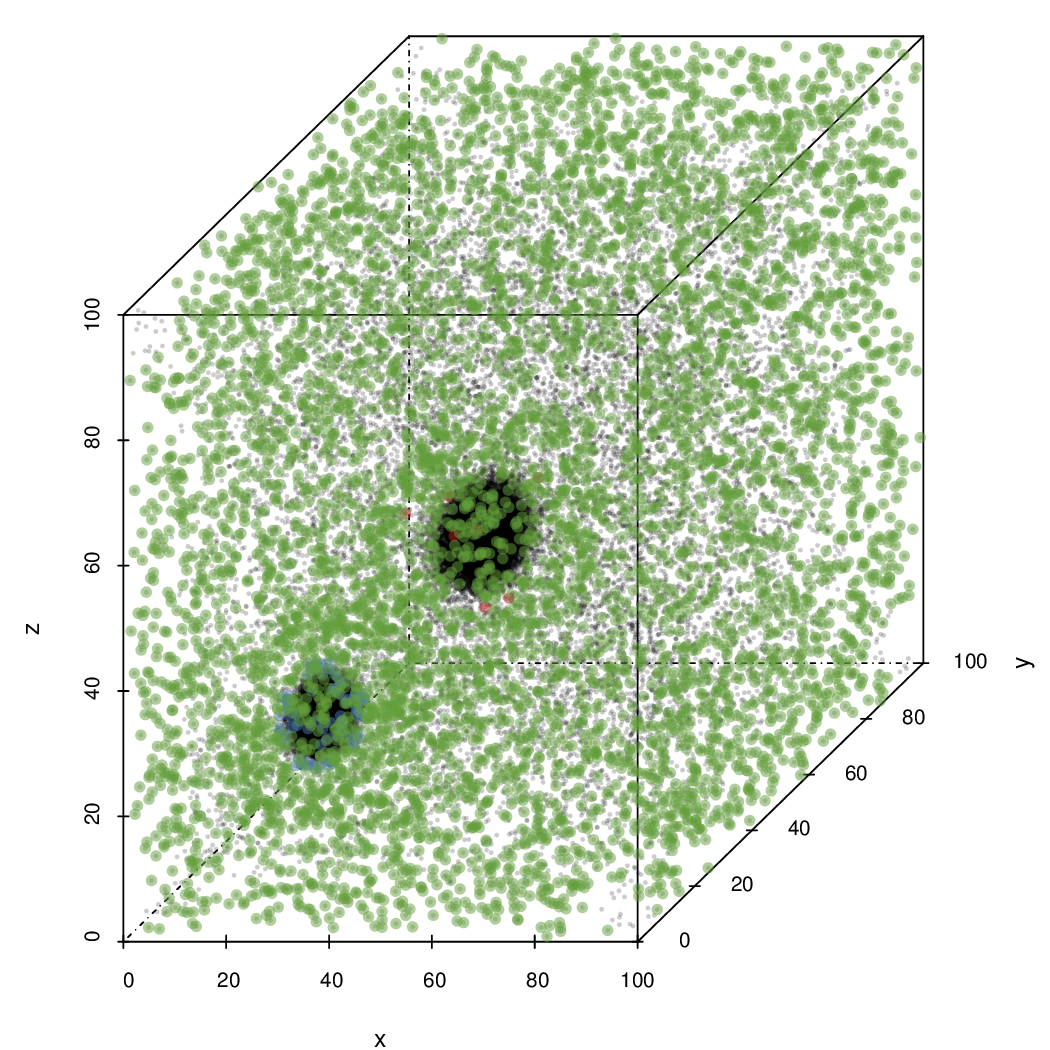
\includegraphics[keepaspectratio=true, width=\textwidth, height=0.23\textheight]{discussion/img/ferdosi_2_60000_anisotropy.png}
					\caption{\ferdosiTwo [\num{2.215970619635167e+00}, \num{5.678002691654005e+00}]}
					\label{fig:discussion:anisotropy:ferdosi2}
				\end{subfigure}
				\begin{subfigure}{0.23\textwidth}
					\centering
					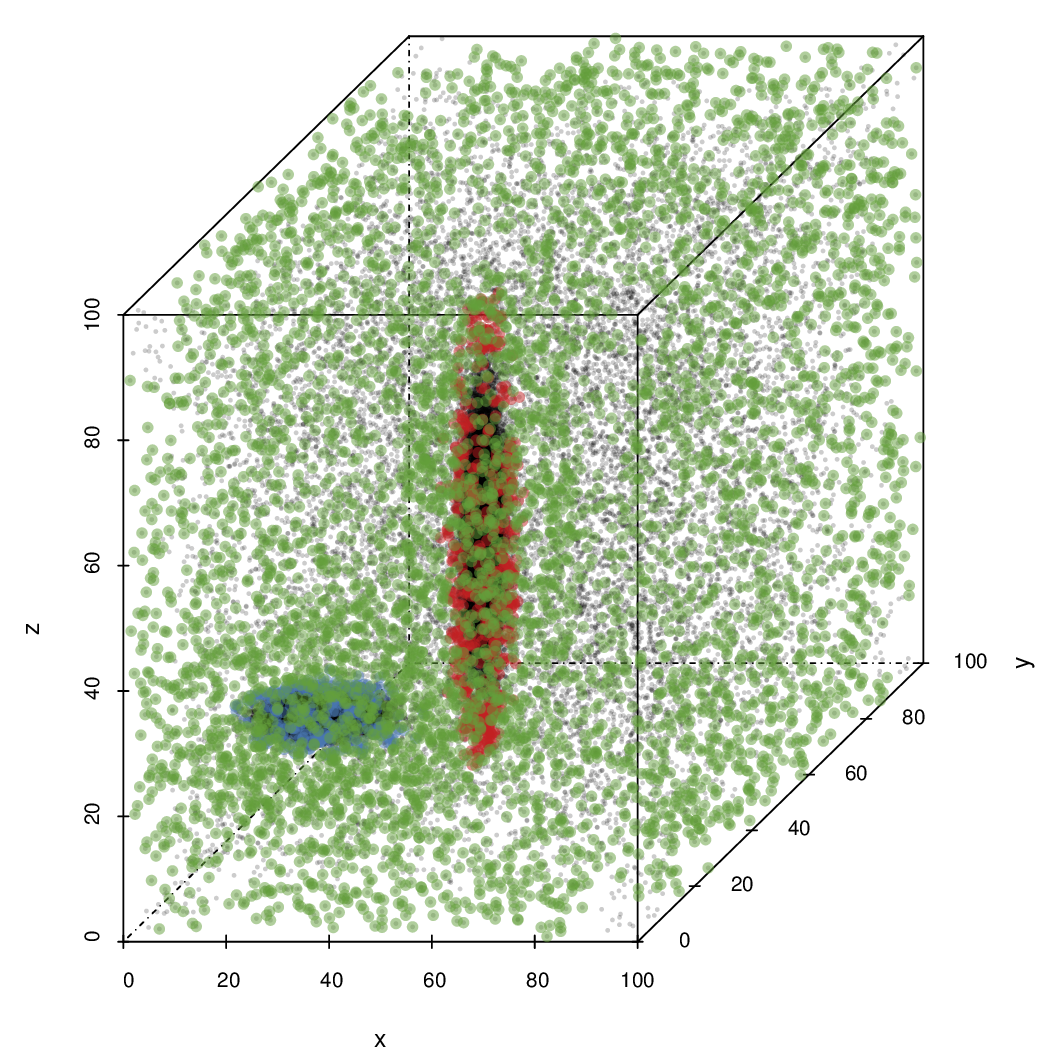
\includegraphics[keepaspectratio=true, width=\textwidth, height=0.23\textheight]{discussion/img/baakman_2_60000_anisotropy.png}
					\caption{\baakmanTwo [\num{2.463414286522871e+00}, \num{7.134567710248723e+00}]}
					\label{fig:discussion:anisotropy:baakman2}
				\end{subfigure}	
				\begin{subfigure}{0.23\textwidth}
					\centering
					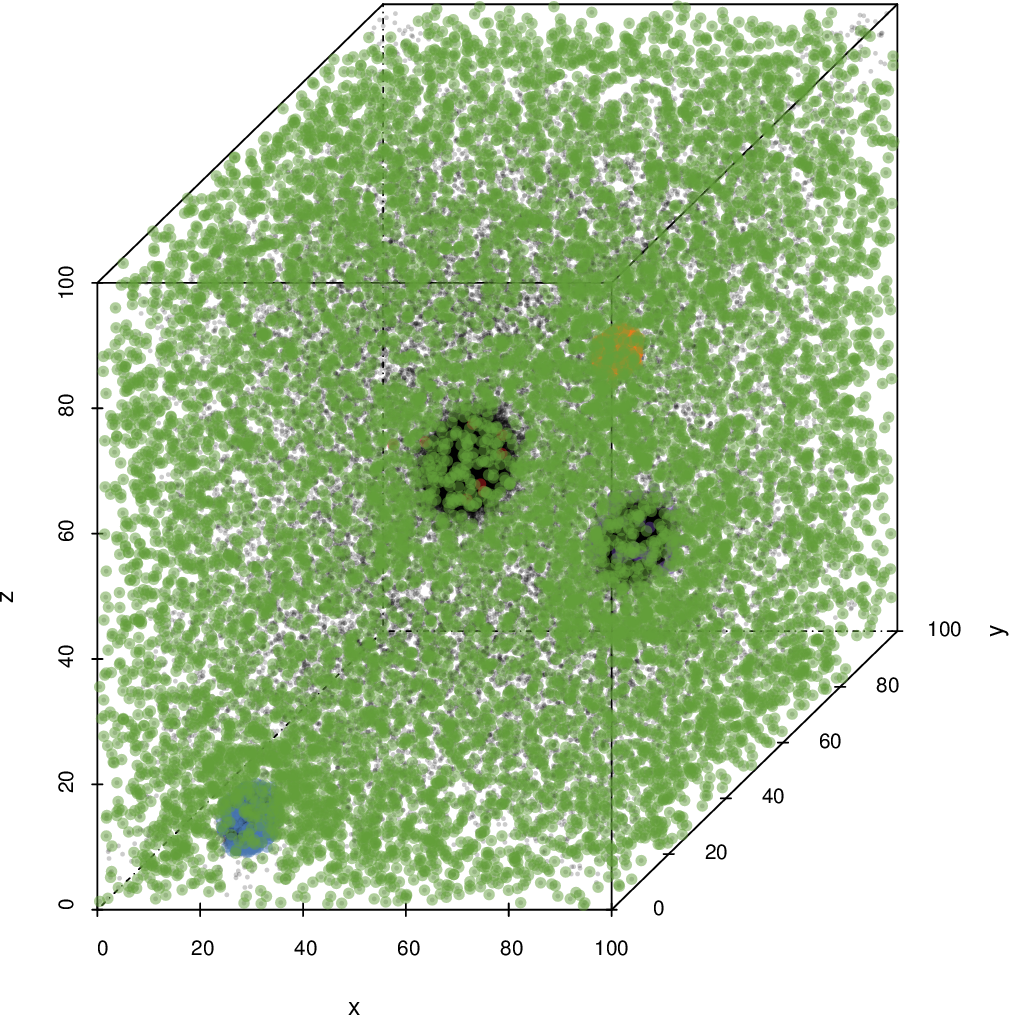
\includegraphics[keepaspectratio=true, width=\textwidth, height=0.23\textheight]{discussion/img/ferdosi_3_120000_anisotropy.png}
					\caption{\ferdosiThree [\num{2.138909227329211e+00}, \num{8.855946762727447e+00}]}
					\label{fig:discussion:anisotropy:ferdosi3}
				\end{subfigure}		
				\begin{subfigure}{0.23\textwidth}
					\centering
					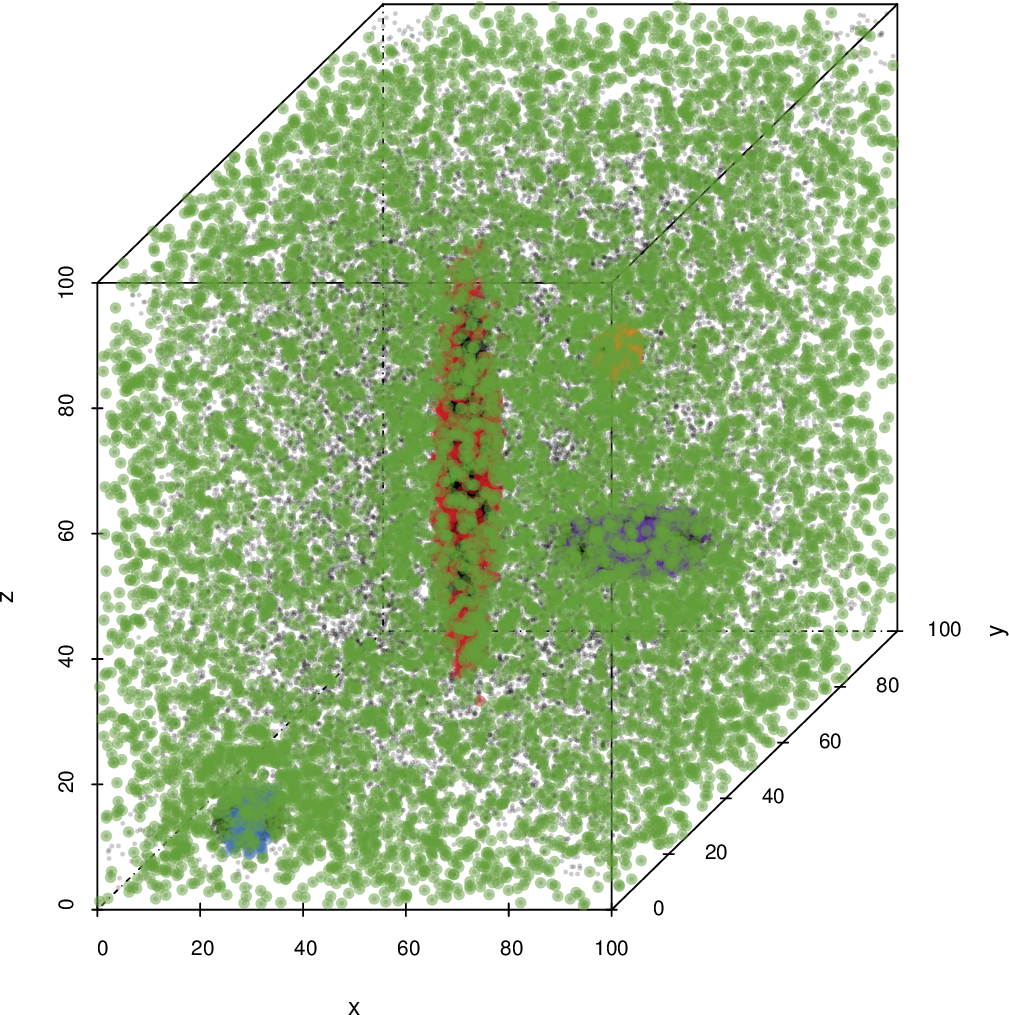
\includegraphics[keepaspectratio=true, width=\textwidth, height=0.23\textheight]{discussion/img/baakman_3_60000_anisotropy.png}
					\caption{\baakmanThree [\num{2.316497642958064e+00}, \num{8.855946762727445e+00}]}
					\label{fig:discussion:anisotropy:baakman3}
				\end{subfigure}			
				\caption{Scatter plot of datasets
					\subref{fig:discussion:anisotropy:ferdosi2} \ferdosiTwo, %
					\subref{fig:discussion:anisotropy:baakman2} \baakmanTwo, %
					\subref{fig:discussion:anisotropy:ferdosi3} \ferdosiThree, and %
					\subref{fig:discussion:anisotropy:baakman3} \baakmanThree. %
					The points that have an anisotropy in the \nth{90} percentile are shown larger and in the color of the component they were drawn from. The range of the anisotropy of the kernels of the emphasized points in shown below each plot.}
				\label{fig:discussion:anisotropy:multisphere}
			\end{figure}			
			% General Introduction
			\Cref{fig:discussion:anisotropy:multisphere} emphasizes the points with the most anisotropic kernels in the dataset \ferdosiTwo through \baakmanThree. 
			% Ferdosi 2
				% Same observations as for ferdosi 1, present percentages
				In the plot associated with dataset \ferdosiTwo we observe the same shells of high anisotropy kernels of points sampled from the noise around the Gaussian components as in dataset \ferdosiOne. Another similarity between these two datasets is that very few points sampled from the Gaussian component have a kernel with high anisotropy; \percentage{1.453877} and \percentage{0.1169786} of the first and second Gaussian component, respectively. 
				% F2G1 vs F2G2
				We contribute the difference in the number of highly anisotropic kernels associated with data points sampled from the two Gaussian components to the difference in density between the two Gaussian components.
			% Baakman 2
				% More points near the Gaussian anisotropic
				Comparing \cref{fig:discussion:anisotropy:ferdosi2,fig:discussion:anisotropy:baakman2} we find that the increase in anisotropy of the kernel has causes \percentage{4.328209} and \percentage{8.656417} of the kernels with high anisotropy to be associated with a point sampled from `Trivariate Gaussian 1' and 2, respectively. 
			% Ferdosi 3
				% G1 and G3 have anisotropic kernels. 
				Interestingly in dataset \ferdosiThree, two of the four spherical Gaussians, \ie `Trivariate Gaussian ' are associated with respectively \percentage{1.404095} and \percentage{2.223151} of the highly anisotropic kernels.
				% Relate to results: components with highest sd, lowest means, lower density -> larger variation in anisotropy
				Comparing the mean kernel anisotropy in \cref{tab:results:multiSphere:anisotropy} we find that compared to the other Gaussian components in \ferdosiThree, these two component have a relatively low mean. However their standard deviations are higher, suggesting that in these denser components some kernels are extremely anisotropic, whereas others are near to isotropic. We contribute this difference within the points sampled from a Gaussian component to difference in physical density of the data points nearer and father away from the mean as we did for dataset \ferdosiOne and \baakmanOne.
				% Why G1 and G3 and not G2 and G4? 
				Component one and four of dataset \ferdosiThree differ from the other Gaussian components in two aspects: firstly they have a relatively dense and secondly they are placed near the boundaries of the dataset. 
					% G1/G3 are placed near the  border of the dataset, contrast with results of F3Noise?
					\Cref{fig:discussion:ferdosi3Noise:anisotropy} shows that distance to the boundaries do not explain the difference in anisotropy of the kernel as in that figure the first and third component of \ferdosiThreeNoise have more anisotropic kernels than the other components.
					% G1/G3 have lower covariance:
					The first explanation fits with the observations from \cref{s:results} that components with a higher density have a higher anisotropy.
			% Baakman 3
				In dataset \baakmanThree we observe the same effect as in \ferdosiThree but stronger; from the points with the most anisotropic kernels more are sampled from the two densest Gaussian component than from the others. 

		% Some general conclusion
		\Cref{fig:discussion:anisotropy:singleSphere,fig:discussion:anisotropy:multisphere} show that the overwhelming majority of the points with a relative highly anisotropic kernel are sampled from the `Uniform random background'. We contribute this to the covariance detecting fine, random structures in the noise, that give the impression of anisotropy where there is none.

% Denser component -> higher anisotropy of kernels
% AND Higher anistropy in component -> higer anisotropy in associated kernels
% AND Denser comonent -> lower MSE
	% Introduce the dataset A1 and A2, same anisotropy different density, what do we observe, what does it say about this correlation.
% Refer back to the difference between G1/G3 versus G2/G4 in F3.

% Lack of difference in anisotropy between F3 and B3 in orange (‘Trivariate Gaussian 3’) component. 

% Some conclusion